\documentclass[a4paper,12pt]{article}

\usepackage{graphicx}

\begin{document}
    \section*{Dynamics}
        \subsection*{Exercise \#1}
	Consider the wheel shown in the picture, acted on by two forces. What
	magnitude of the force F2 will be required for the wheel to be in rotational
	equilibrium?

	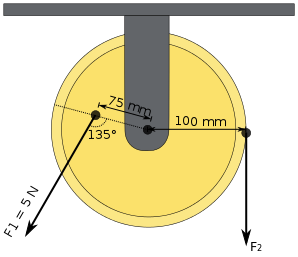
\includegraphics{img/torque-angular-momentum-ex1.png}
\end{document}
